% Created 2022-07-01 Fri 11:45
% Intended LaTeX compiler: pdflatex
\documentclass[11pt]{article}
\usepackage[utf8]{inputenc}
\usepackage[T1]{fontenc}
\usepackage{graphicx}
\usepackage{longtable}
\usepackage{wrapfig}
\usepackage{rotating}
\usepackage[normalem]{ulem}
\usepackage{amsmath}
\usepackage{amssymb}
\usepackage{capt-of}
\usepackage{hyperref}
\author{Pietro Visconti, Diego Passarella, Tudor Croitor}
\date{\today}
\title{Progetto PCTO Ca'Foscari}
\hypersetup{
 pdfauthor={Pietro Visconti, Diego Passarella, Tudor Croitor},
 pdftitle={Progetto PCTO Ca'Foscari},
 pdfkeywords={},
 pdfsubject={},
 pdfcreator={Emacs 28.1 (Org mode 9.5.2)}, 
 pdflang={English}}
\begin{document}

\maketitle
\tableofcontents


\section{Descrizione progetto}
\label{sec:orga97862f}
La web application permette la gestione dei corsi riguardanti le \textbf{attività PCTO} dell'Università.

\subsection{Funzionalità principali}
\label{sec:org36f7484}

\subsubsection{Registrazione ed accesso alla web application}
\label{sec:org2b92bdb}
All'interno dell'applicazione è possibile registrarsi come \textbf{studente} o come \textbf{professore}.
Nella procedura di registrazione vengono richiesti Nome, Cognome, Data di nascita, Email, Password (e conferma password) ed infine la tipologia di utente.

Al termine della registrazione, tuttavia, sarà possibile accedere alla propria area riservata solo dopo aver aperto il \textbf{link di attivazione} (spiegato meglio in seguito) che verrà inviato alla email inserita durante la procedura. Questa è una forma di sicurezza che viene adottata con lo scopo di prevenire che l'utente possa registrarsi con una email a cui egli non ha accesso. Una volta attivato l'account, si potrà accedere alla web application tramite il form di login, inserendoci email e password.

Come anticipato, una volta premuto il tasto "Registrati" viene automaticamente inviata una email all'indirizzo specificato nel form, a cui viene passato come parametro un \textbf{token alfanumerico univoco}. Tale token viene poi associato all'utente nella tabella tokens. Nel frattempo, viene inserito l'utente nella tabella users, nella quale viene salvato un flag \textbf{"is\textsubscript{active}"} per verificare che l'utente abbia attivato il proprio account. Fintanto che il flag rimane a False, l'utente non può accedere alla web application. Subito dopo che l'utente ha cliccato il link di attivazione, viene verificato che il token presente nei parametri del link e quello già salvato nel database corrispondano: in caso positivo, il flag "is\textsubscript{active}" viene impostato a True e l'utente potrà accedere.

Nella procedura di registrazione dei professori esiste un controllo addizionale: viene verificato che il \textbf{dominio dell'email} inserita nel form sia "unive.it" per accertarsi che quantomeno l'utente faccia parte dell'Università.

Tutti gli utenti possono eventualmente effettuare il \textbf{logout} dalla web application.

\subsubsection{Accesso come Professore}
\label{sec:org9d96575}
Se l'utente effettua l'accesso in qualità di professore avrà a diposizione:
\begin{itemize}
\item Sezione \textbf{Profilo}, in cui verranno visualizzate tutte le informazioni personali.
\item Sezione \textbf{Gestione Corsi}, una dashboard in cui sono esposti tutti i corsi creati dall'utente e visualizzarne le specifiche: Titolo, Categoria, Data di creazione, Numero di iscrizioni massimo e la sezione "Azioni", spiegata in seguito.
\item Sezione \textbf{Crea nuovo corso}, nella quale è possibile appunto creare un nuovo corso, inserendo queste caratteristiche: Titolo, Descrizione, Massimo numero di partecipanti, Minimo numero di partecipanti, Minimo numero di lezioni, Durata delle lezioni, Categoria.
\item Per ogni corso, sezione \textbf{Azioni}: sono presenti dei bottoni per accedere alle sezioni Lezioni, Informazioni Corso, Modifica Corso.
\item Sezione \textbf{Lezioni}, in cui l'utente può aggiungere nuove lezioni relative al corso che sta modificando.
Per ogni lezione sono richiesti Descrizione, Data, Orario, Modalità, Edificio, Aula.
\item \label{org49fa94f}Sezione \textbf{Informazioni Corso}, in cui viene presentata un'overview del corso in questione: sono presenti la descrizione, le lezioni presenti (con possibilità di aggiungerne), la \textbf{mini-mappa} con il marker che indica il luogo di svolgimento della lezione più vicina temporalmente e la lista di studenti partecipanti.
\item Sezione \textbf{Modifica Corso}, in cui è possibile modificare in tempo reale (senza dover ricaricare la pagina) le informazioni relative al corso in questione.
\end{itemize}

\subsubsection{Accesso come Studente}
\label{sec:org9abdb27}
Se l'utente effettua l'accesso in qualità di studente, avrà a disposizione:
\begin{itemize}
\item Sezione \textbf{Tutti i corsi}, in cui viene esposta una lista di tutti i corsi creati dai professori suddivisi in categorie. Per ogni corso, lo studente può visualizzarne i dettagli, tra cui Titolo, Descrizione, Creatore, Data di creazione, Numero di posti e il Numero di posti disponibili.
\item Sezione \textbf{I miei corsi}, nella quale vengono mostrati i corsi ai quali lo studente è iscritto. Viene data la possibilità di cancellare la propria iscrizione e di visualizzare i dettagli relativi al corso (vedi \hyperref[org49fa94f]{Informazioni Corso}).
\end{itemize}


\subsection{Progettazione}
\label{sec:org8e47861}

\subsubsection{Schema concettuale}
\label{sec:org24d68f8}
\begin{center}
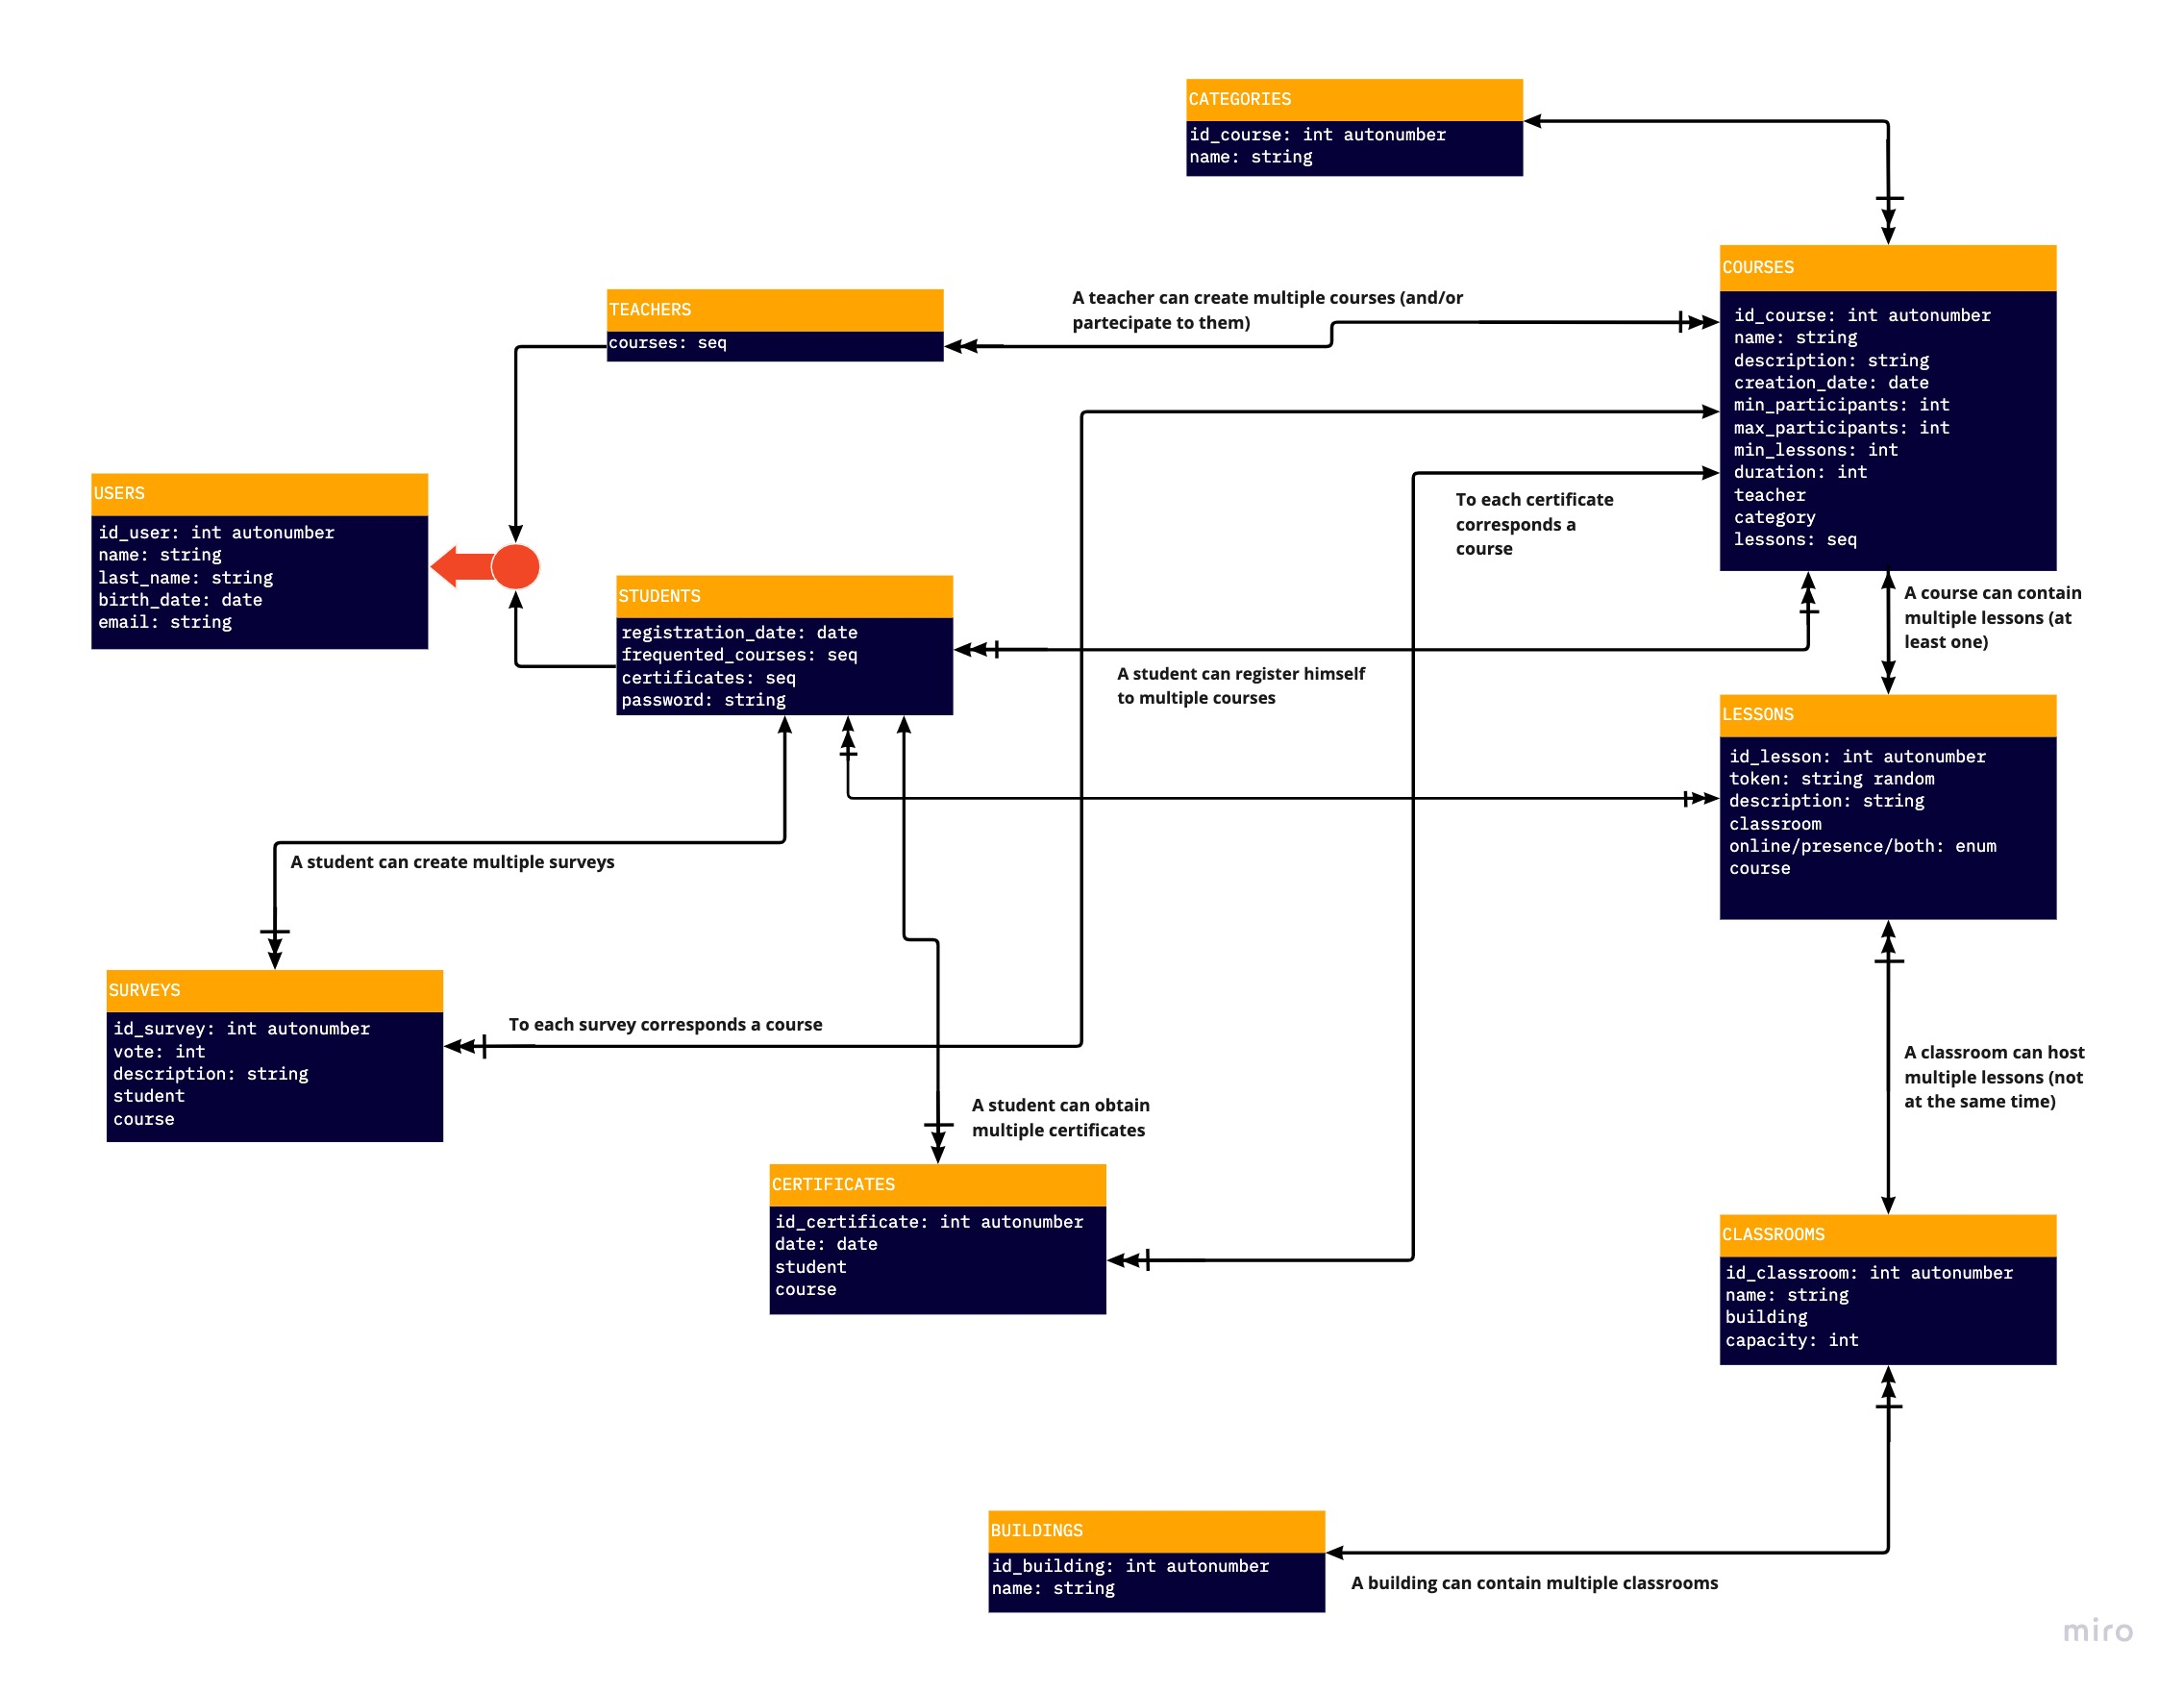
\includegraphics[width=.9\linewidth]{./resources/conceptual_scheme.jpg}
\end{center}

\begin{quote}
\textbf{NOTA}: Attualmente le funzionalità riguardanti le tabelle \textbf{Surveys} e \textbf{Certificates} non sono ancora state implementate.
\end{quote}

Nello schema concettuale qui mostrato, si evidenziano le seguenti relazioni:
\begin{enumerate}
\item Gli utenti si suddividono in Studenti e Professori.
\item Ad ogni utente viene associato un token (nella tabella tokens).
\item Ogni Professore può creare molteplici corsi.
\item Ogni Studente può partecipare a molteplici corsi.
\item Ad ogni corso corrisponde una categoria.
\item Ad ogni corso sono associate molteplici lezioni.
\item Uno studente può partecipare a più lezioni.
\item Uno studente può partecipare a molteplici sondaggi.
\item Uno studente può possedere molteplici certificati di partecipazione.
\item A ogni lezione viene associata un'aula, e all'aula un edificio
\end{enumerate}

\subsubsection{Schema logico}
\label{sec:orge3454aa}
\begin{center}
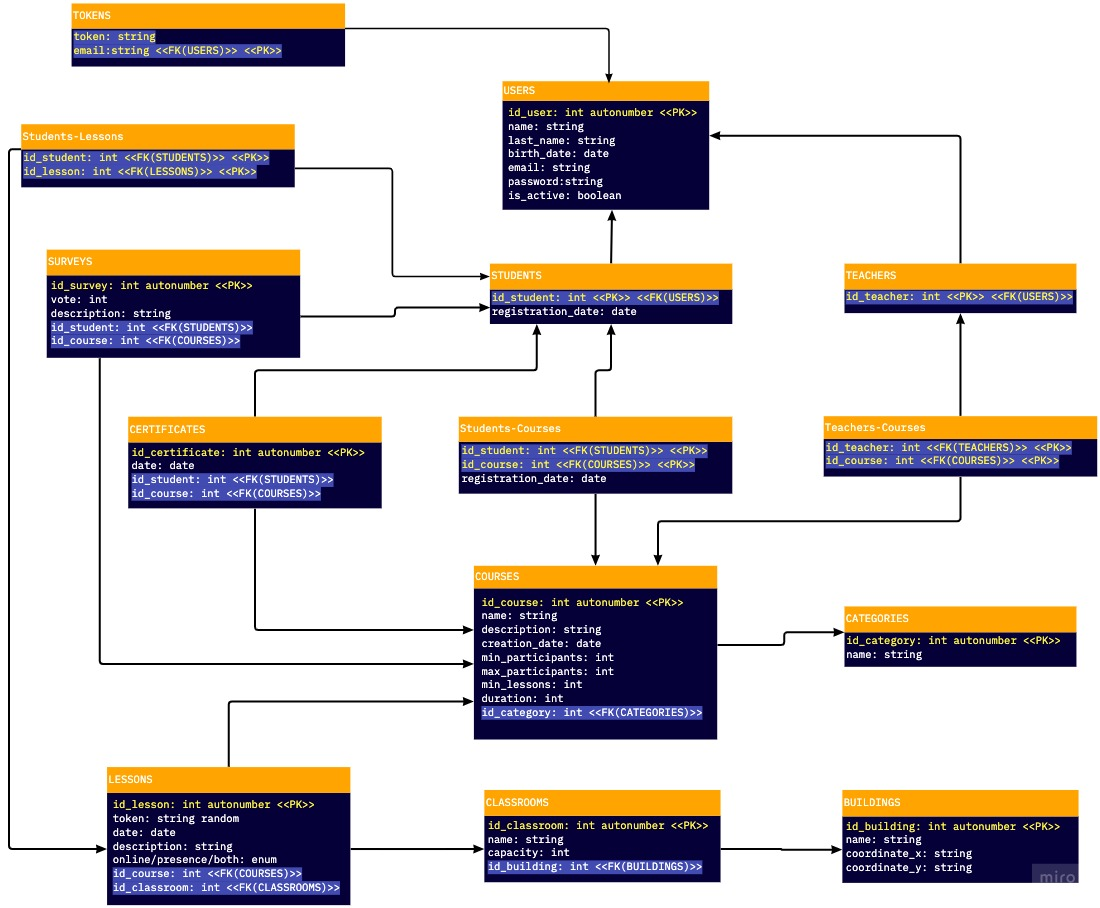
\includegraphics[width=.9\linewidth]{./resources/relational_scheme.jpg}
\end{center}

\subsection{Scelte progettuali}
\label{sec:org1ccc56c}

\subsubsection{Politiche di integrità dei dati}
\label{sec:org4ecf8b0}
Per prevenire eventuali incongruenze durante l'inserimento/aggiornamento di nuovi dati all'interno delle tabelle, sono stati effettuati dei controlli tramite i \textbf{check constraints} su attributo o tupla.

Alcuni esempi:

\begin{center}
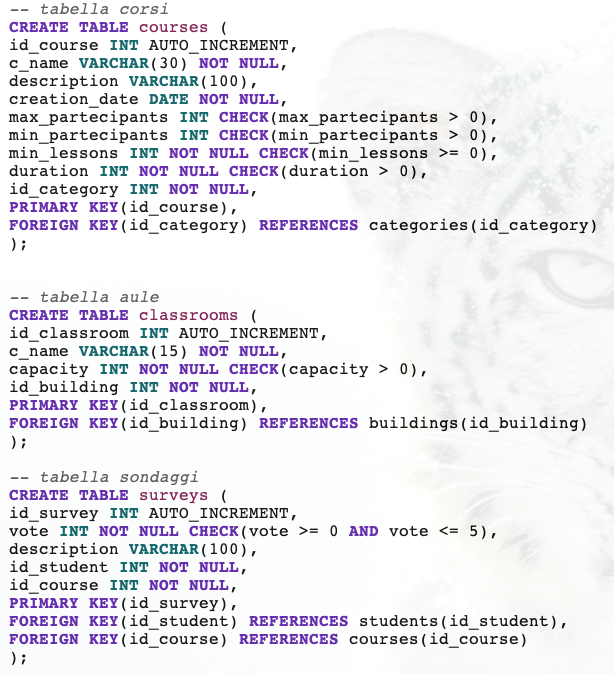
\includegraphics[width=.9\linewidth]{./resources/create_table.png}
\end{center}

Altri controlli più complessi, invece, sono stati effettuati tramite codice, per renderli più capibili e flessibili.

Esempio in cui viene verificato che l'aula inserita non sia già occupata da un'altra lezione nello stesso orario:

\begin{center}
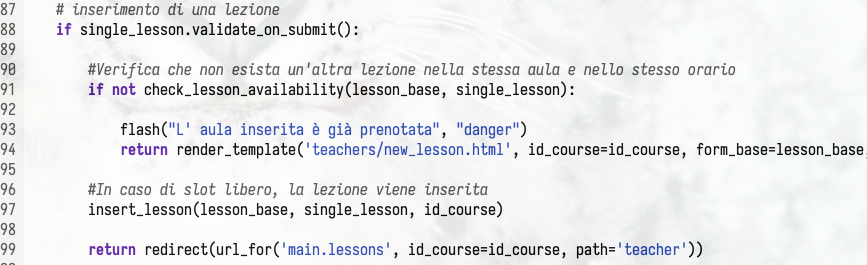
\includegraphics[width=.9\linewidth]{./resources/insert_lesson.png}
\end{center}

\subsubsection{SQLAlchemy ORM}
\label{sec:orgb6066d3}

E' stato scelto di adottare la tecnologia \textbf{Object-Relational-Mapping} in quanto permette di incapsulare le tabelle e le rispettive relazioni in classi, rendendo il codice e le query facili da scrivere e da capire. Un altro aspetto importante da sottolineare è che SQLAlchemy ORM garantisce la \textbf{protezione da SQL-Injection}.

Anche le relazioni tra le classi ORM sono state affidate completamente a SqlAlchemy: in questo modo ogni modifica fatta allo schema del database viene riflessa immediatamente nelle classi python. Questo garantisce protezione da eventuali bug dovuti ad una modifica di attributi/relazioni, \textbf{rendendo sicuro ogni cambiamento} allo schema relazionale.

Esempio:

\begin{center}
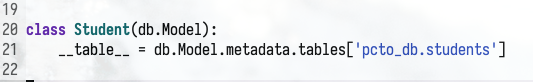
\includegraphics[width=.9\linewidth]{./resources/orm.png}
\end{center}

\subsection{Scelte tecnologiche}
\label{sec:org8ddb3fe}

\subsubsection{JQuery?}
\label{sec:orgbe822ac}

\subsubsection{Folium?}
\label{sec:org9c3e58a}
\end{document}